\chapter{Aufbau und Ablauf von Testprojekten}
\label{cha:Konzept}

Dieses Kapitel befasst sich mit den Testabläufen in einem Softwareprojekt. Diese Abläufe finden in unterschiedlichen Phasen eines Softwareprojekts statt und werden von unterschiedlichen Personengruppen durchgeführt. Diese Kapitel gibt einen Einblick in diese Abläufe und beschreibt auch die Schwierigkeiten, die es in einem Testprojekt zu bewältigen gibt. Im zweiten Abschnitt wird die Evolution der Testautomatisierung beschrieben. Dabei werden unterschiedliche Testansätze vorgestellt, welche sich über die Zeit entwickelt haben. Einer diese Testansätze stellt die Basis für das Rayden-System dar.

\section{Ablauf eines Testprojekts}

In einem Softwareentwicklungsprojekt gibt es nicht nur die Test-Phase, in welcher die Testabteilung eine wichtige Rolle spielt. Die Testabteilung ist in den meisten Phasen eines Entwicklungsprojekts involviert. Um die gesamten Testaufgaben in einem großen Projekt zu koordinieren, wir oft ein Testprojekt aufgesetzt. In einem Testprojekt werden alle Aktivitäten rund um die Qualitätssicherung vereint. Diese Aktivitäten beschränken sich aber nicht nur auf die Testabteilung. Es müssen auch Personen aus der Fachabteilung und der Entwicklungsabteilung eingebunden werden. Diese Schnittstellen zwischen den einzelnen Abteilungen bieten eine große Herausforderung für die Testmanagerin oder dem Testmanager.

\SuperPar
Die Komponenten- und Integrationstests werden in diesem Abschnitt nicht behandelt, da diese Testaktivitäten primär in der Entwicklungsabteilung durchgeführt wird. Der Fokus der Testabteilung liegt auf den manuellen und automatisierten Abnahmetests der Anwendung.

\SuperPar
In den nachfolgenden fünf Unterabschnitten werden die einzelnen Aufgaben in eine Testprojekt beschrieben. Es wird beschrieben, wie Testfälle entwickelt werden und zu welchem Zeitpunkt in einem Softwareprojekt welche Testaktivitäten ablaufen.

\subsection{Rollen in einem Testprojekt}

Das Testprojekt besteht aus einer bunten Mischung an unterschiedlichen Personen. Die Verantwortung in einem Testprojekts trägt die Testmanagerin oder der Testmanager. Diese Person ist für die Koordination des Projekts zuständig und bildet die Schnittstellen zu anderen Abteilungen. Eine Schnittstellen besteht zu der Fachabteilung. Von der Fachabteilung werden die Anwendungsfälle geliefert welche in weiterer Folge in der Testabteilung umgesetzt werden. Für die Umsetzung der Testfälle sind die Testerinnen und die Tester zuständig. Für die Automatisierung von Testfällen besteht eine Schnittstelle zu der Entwicklungsabteilung, falls die Testabteilung über keine eigene Entwicklerinnen oder Entwickler verfügt.

\subsection{Testfall}

Während der Konzeptionsphase in einem Entwicklungsprojekts werden Anforderungen von der Fachabteilung aufgenommen. Aus diesen Anforderungen werden Anwendungsfälle für das gesamte Projektteam abgeleitet. In der Testabteilung werden aus den Anwendungsfälle Testfälle entwickelt. Die Testfälle werden benötigt, um einen Überblick zu bekommen, welche Bereiche einer Software getestet werden müssen. In einem Testfall wird beschrieben, wie der Anwendungsfall zu testen ist und wie das erwartete Ergebnis aussieht. Da diese Aufgabe wichtig ist und einen hohen Kommunikationsaufwand bedeutet, werden die Testfälle größtenteils von der Testmanagerin oder dem Testmanager durchgeführt. In großen Projekten wird diese Arbeit auch von erfahrenen Testerinnen oder Testern durchgeführt. 

\subsection{Manuelle Abnahmetests für Testfälle}

Die Testfälle bestehen aus einer groben Beschreibung des zu testenden Anwendungsfall. Weiters beinhaltet ein Testfall eine Schritt für Schritt Anweisung, wie der Testfall ausgeführt werden soll. Ein Testfall wird in der erste Phase von einer Testerin oder einem Tester durchlaufen. Für die Zuteilung der Testfälle ist die Testmanagerin oder der Testmanager zuständig. 

\subsection{Automatisieren von manuellen Abnahmetests}

In regelmäßigen Abständen sieht sich die Testmanagerin oder der Testmanager die Ausführungshäufigkeit von manuellen Tests an. Werden manuelle Tests sehr oft durchgeführt, wird dieser Test automatisiert. Bei der Automatisierung werden die manuellen Schritte mithilfe von einem Test-\enword{Framework} automatisiert. Durch die Automatisierung spart die Testabteilung Zeit und kann somit schneller Ergebnisse über die Qualität der Anwendung liefern.

\subsection{Testdokumentation}

Der große Vorteil von sauber spezifizierten Testfällen ist, dass man keine zusätzliche Testdokumentation benötigt. Wenn die Testfälle sorgfältig beschrieben sind und auch gewartet werden, dienen diese als Testdokumentation. Wurden Testfälle automatisiert, kann es passieren, dass die Implementierung des Testfall über die Zeit nicht mehr mit der Beschreibung übereinstimmt. Ein wichtiges Ziel bei der Automatisierung ist es daher, dass man die Testdokumentation aktuell hält. Aus diesem Grund gibt Automatisierungsansätze, welche Versuchen, die manuellen Testfälle direkt zu automatisieren. Einige dieser Ansätze werden im nächste Abschnitt \ref{cha:evolution} erklärt. Ein anderer Vorteil bei diesen Ansätzen ist, dass man die automatisieren Tests noch immer manuell ausführen kann. Diese Eigenschaft kann für Verifikationen von Ergebnissen sehr wichtig sein.

\section{Evolution der Testautomatisierung}
\label{cha:evolution}

Die Automatisierung von Abnahmetests hat sich über die Zeit einen starken Wandel unterzogen. In diesem Bereich hat es eine ähnliche starke Entwicklung wie bei den Softwareentwicklungstechniken gegeben. Im Jahr 2009 haben Jeff Hinz und Martin Gijsen eine Artikel \cite{Hinz09} über die Evolution der Testautomatisierung veröffentlicht. In diesem Artikel teilen die beiden Autoren die Entwicklung der Testautomatisierung in fünf Generationen ein. Jede Generation zeichnet sich durch eine spezielle Technik aus, wie die Test entwickelt werden. 

\begin{figure}
\centering
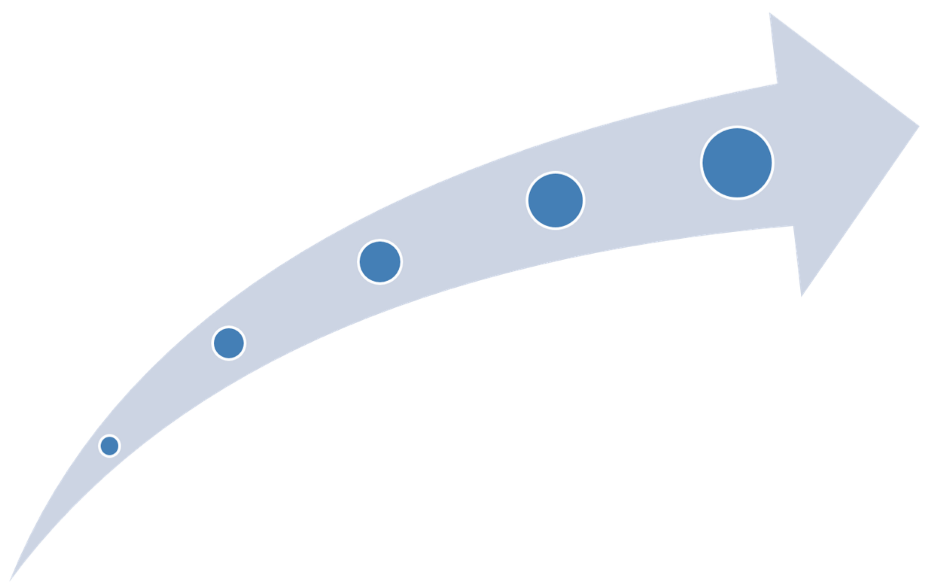
\includegraphics[width=0.9\textwidth]{EvolutionVonTest.png}
\caption{Die fünf Generationen von Testtechniken}
\label{fig:testEvolution}
\end{figure}

\SuperPar
Die Abbildung \ref{fig:testEvolution} zeigt die einzelnen Entwicklungsstufen. In den nächsten Abschnitten werden die Techniken vorgestellt und auf die Vorteile und Nachteile eingegangen.

\subsection{Erste Generation - \enword{Record-Replay}}

Die erste Generation von Testtechniken sind die \enword{Record-Replay}-Ansätze. Dieser Ansatz besteht aus zwei Phasen. In der ersten Phase wird mithilfe einer Analyse-Software die Aktionen der Benutzerin oder des Benutzers mit der Anwendung aufzeichnet. Dabei werden typischerweise die Mausbewegungen und die Tastatureingaben aufgezeichnet. In der zweiten Phase werden die aufgezeichneten Aktionen mit einer speziellen Software wieder abgespielt. Die Testsoftware beinhaltet dazu spezielle Maus- und Tastatur-Treiber, um die aufgezeichneten Aktionen wiedergeben zu können.

\SuperPar
Der große Vorteil bei dieser Methode ist die Einfachheit. Zum Aufzeichnen von Tests muss die Testerin oder der Tester den Anwendungsfall durcharbeiten und im Hintergrund werden die Aktionen aufgezeichnet. Für diese Testtechnik werden keine speziellen Fähigkeiten benötigt. Jedoch hat diese Technik einen massiven Nachteil. Sobald sich die zu testende Anwendung nur marginal an der Oberfläche ändert, funktioniert diese Testmethode nicht mehr. Auch müssen die Tests immer mit der selben Bildschirmauflösung ausgeführt werden, um die Aktionen korrekt wiedergeben zu können. Ein weiterer Nachteil ist, dass sobald man einen Test ändern möchte, muss man den gesamten Test neu aufzeichnen.

\subsection{Zweite Generation - \enword{Functional Decomposition}}

Bei \enword{Functional Decomposition} werden die Tests in einzelne Testsequenzen zerteilt. Mit dieser Technik konnten langen unleserliche Test in handliche Sequenzen zerteilt werden. Die Methode erlaubt auch die Wiederverwendung von Sequenzen in anderen Tests. Durch einen hohen Wiederverwendungsgrad kann die Größe des Testprojekts stark reduziert werden. Ein weiterer positive Effekt kann man in der Wartbarkeit des Testprojekts feststellen. Durch die Reduktion der Test wird auch der der Wartungsaufwand geringer.

\SuperPar
Mit dieser Testmethode war es nun auch möglich, Bibliotheken mit Testfunktionen für ein Testprojekt anzulegen. 

\subsection{Dritte Generation - \enword{Data-Driven Testing}}

In der dritten Generation von Testmethoden wurde ein großes Augenmerk auf die Testdaten gelegt. In den vorgehenden Testtechniken lag der Fokus auf der Erstellung und Wartung von Testprojekten. Dabei mussten auch schon Testdaten verwendet werden, aber der Stellenwert war nicht hoch. Die Testdaten stehen dafür nun in dieser Generation im Mittelpunkt. Man erkannte, dass man oft die selbe Testsequenz durchläuft, aber jedes Mal andere Daten verwendet. Diese Testtechnik wird stark für datenzentrierten Anwendungen verwenden. 

\SuperPar
Bei einem \enword{Data-Driven-Testing} werden im Test keine konkrete Werte verwendend. Statt dessen werden Platzhalter (Variablen) im Test eingebaut. Bei der Ausführung eines Tests werden die Platzhalter mit einem Wert aus einer Datenquelle verbunden. Als Datenquelle können Dateien wie auch Datenbanken dienen. Mit dieser Technik, kann man ein und denselben Test mit unterschiedlichen Daten ausführen. 

\subsection{Vierte Generation - \enword{Keyword-Driven Testing}}

In der vierten Generation von Testmethoden werden die Testdaten noch weiter in den Mittelpunkt gestellt. Bis zu diesem Zeitpunkt wurden die Test entweder mithilfe eines \enword{Record-Replay}-Ansatzes aufgezeichnet oder in einer Programmiersprache entwickelt. Der \enword{Record-Replay}-Ansatz war einfach und auch von nicht technisch versierten Personen zu benutzen. Jedoch haben diese aufgezeichneten Test ein Zuverlässlichkeitsproblem. Der zweite Ansatz bedingt, dass die Personen aus der Testabteilung Programmierkenntnisse benötigen.

\SuperPar
Bei \enword{Keyword-Driven-Testing} wurden die Tests nun auch als Testdaten angesehen. Mit diesem Ansatz können Tests mit dem gleichen Ansatz wie die Testdaten erstellt und verwaltet werden. Um einen \enword{Keyword-Driven}-Test ausführen zu können, wird ein spezieller Interpreter benötigt. Der Interpreter liest die Tests über eine Datenquelle ein und arbeitet diese ab. Für die Verarbeitung müssen die Tests in einem lesbaren Format für den Interpreter vorliegen. Eine detaillierte Beschreibung liefert Pekka Laukkanen von der Universität von Helsinki in seiner Masterarbeit \cite{Lauk06}. 

\subsection{Fünfte Generation - \enword{Scriptless Automation}}

Die letzte Methode versucht die Testautomatisierung mit einem \enword{Scriptless-Automation}-Ansatz zu vereinfachen. Bei diesem Ansatz wird versucht, dass man aus einer abstrakten Repräsentation eines Tests den Code zu erzeugen. Bei diesem Transformationsvorgang werden Code-Vorlagen und Code-Generatoren verwendet.

\SuperPar
Bei diesem Ansatz wird wiederum versucht, die Größe des Testprojekts zu reduzieren und somit die Wartbarkeit zu erhöhen. Diese Ansatz befindet noch in einer frühen Phase und hat in der Praxis bis jetzt noch keine Relevanz. 

\SuperPar
Im nächsten Abschnitt wird eine Implementierung des \enword{Keyword-Driven-Testing} vorgestellt, welches die Grundlage für das Rayden-System ist.

\section{\enword{Robot-Framework}}

Das \enword{Robot-Framework} \cite{Robot} ist die Umsetzung des \enword{Keyword-Driven-Testing}-Ansatzes und wurde ursprünglich von Nokia Siemens Networks entwickelt. Später wurde das Projekt unter die Apache 2 Lizenz gestellt und veröffentlicht. Das \enword{Robot-Framwork} stellt nicht nur eine technische Basis zur Verfügung, sondern bietet auch ein Vorgehensmodell dafür an. Das Vorgehensmodell wird \enword{Acceptance test-Driven Development} (ATDD) genannt und im Artikel \cite{Lar10} erklärt.

\begin{program}
\begin{JavaCode}
*** Test Cases ***
Anmelden an der PetClinic Anwendung
	[Documentation]	Man meldet sich bei der Anwendung PetClinic mit 
	...             den definierten Daten an. Wenn das Keyword 
	...             erfolgreich ausgeführt worden ist, befindet man 
	...             sich auf der Hauptseite der Webanwendung.
	
	Open Browser	${URL}		${Browser}
	Input Text    user			TestUser
	Input Text		password	secret
	Click Button	login

\end{JavaCode}
\caption{Beispiel von einem \enword{Robot-Framework}-Testfall}
\label{prog:robotTestCase}
\end{program}

\SuperPar
Das \enword{Robot-Framework} verwendet als Testdaten-Format eine Tabulator-Syntax. Dabei werden die Daten durch Tabulatoren getrennt. Die Abbildung \ref{prog:robotTestCase} zeigt einen Testfall, welcher in der Tabulator-Syntax definiert worden ist. In dem Testfall wurde die Selenium-Bibliothek für das \enword{Robot-Framework} verwendet. 

\SuperPar
Das \enword{Robot-Framework} unterstützt die Verwendung von Bibliotheken. In einer Bibliothek können \enword{Keywords} zusammengefasst werden. Das \enword{Robot-Framework} und die Entwickler dahinter stellen eine große Anzahl an vorgefertigten Bibliotheken zur Verfügung. Die vorgefertigten Bibliotheken erleichtern und beschleunigen das Entwickeln von Test enorm. Somit muss man nicht bei jedem neuen Projekt von Null beginnen, sonder kann auf einen Fundus an \enword{Keywords} zurück greifen.

\SuperPar
Ein anderer Vorteil dieser Bibliotheken ist es, dass auch Person ohne technischem Hintergrund dieses \enword{Robot-Framework} verwenden können. Die Bibliotheken sind weitestgehend vollständig, dass man nur selten in die Lage kommt, in der man neue \enword{Keywords} implementieren muss.

\SuperPar
Neben den vielen Vorteil des \enword{Robot-Framework}, gibt es aber auch Nachteile. Ein Nachteil wäre die Tabulator-Syntax. Diese Syntax ist Fehleranfällig und ohne einem speziellen Editor nur mühsam zum lesen. Auch fügt sich die Unterstützung von Kontrollstrukturen nicht optimal in das System ein.

\SuperPar
Das \enword{Robot-Framework} und die identifizierten Probleme bilden den Startpunkt für das Rayden-System, welches im nächsten Kapitel beschrieben wird.

